% !TEX root = INT.tex

\chapter{Signal Region Definition}
\label{chap:SignalRegion}

\indent The kinematic selections in the signal region are designed to reject SM ttbar events, which comprise 70-90 percent of all background in SR.  The same selections are also effective at rejecting sub-dominant backgrounds including $W$+jets, single top, $Z$+jets and QCD multijet backgrounds.  This chapter first builds physical intuition on the dominant SM ttbar in section \ref{sec:SR:physical}.  A brief recap of the ISR reconstruction algorithm is given in section \ref{sec:SR:Definitions}.  The SR kinematic selections are defined in section \ref{sec:SR:Selections}.  The section also goes into detail on the background rejection power of each SR selection. Lastly the SR yields and background composition are covered in section \ref{sec:Bkg:Yields} and \ref{sec:Bkg:Compositiion}.  \\

\section{Physical Intuition on how Signal Region Selections Reject SM Background}
\label{sec:SR:physical}

\indent The zero lepton SR is designed specifically to reject the dominant ttbar background.  The SR's design choice and signal and ttbar kinematics are summarized in this section.  The SR's effect on sub-dominant backgrounds are also described near the end of the section. More detail on each SM background, including background estimation techniques, can be found in chapter \ref{chap:backgrounds}. \\

\indent 95 percent of all ttbar which survive SR selection decay via the single hadronic tau and single lepton decay channels.  SM ttbar that decays via the fully hadronic decay channel generates no little intrinsic $\MET$ and is negligible in SR.  Therefore, understanding ttbar specifically require us to understand the single lepton decay channel where the leptonic top can decay via an electron, muon or tau. \\

\indent It is important to note that a top decay cannot generate a neutrino with 250 $\gev$ $\pt$ if the top decays at rest.  Therefore, the $\MET > 250 \gev$ requirement essentially forces the leptonic top to be boosted.   \\

\indent  The leptonic top can only gain boost in one of two ways.  Either the leptonic top recoils against the hadronic top in a back-to-back fashion or both tops recoil against strong ISR.  This break down of SM ttbar into two kinematically distinct populations is covered in more detail in section \ref{sec:Bkg:ttbar}.  \\

\indent The thrust axis, the axis that maximizes the amount of back-to-back $\pt$ along it, contains important information in both populations.  In the top/anti-top population, the thrust axis aligns along the top/anti-top back-to-back boost.  In the ttbar+strong ISR population, the thrust axis aligns along the ISR/ttbar back-to-back boost.  \\

\indent Figure \ref{fig:ttbar:3pop} illustrates example events from the two distinct ttbar populations and the stop signal.  We line up all three events according to their thrust axis and the hemisphere containing the $\MET$ displayed in the upper half.  \\

\begin{figure}[h!]
  \centering
	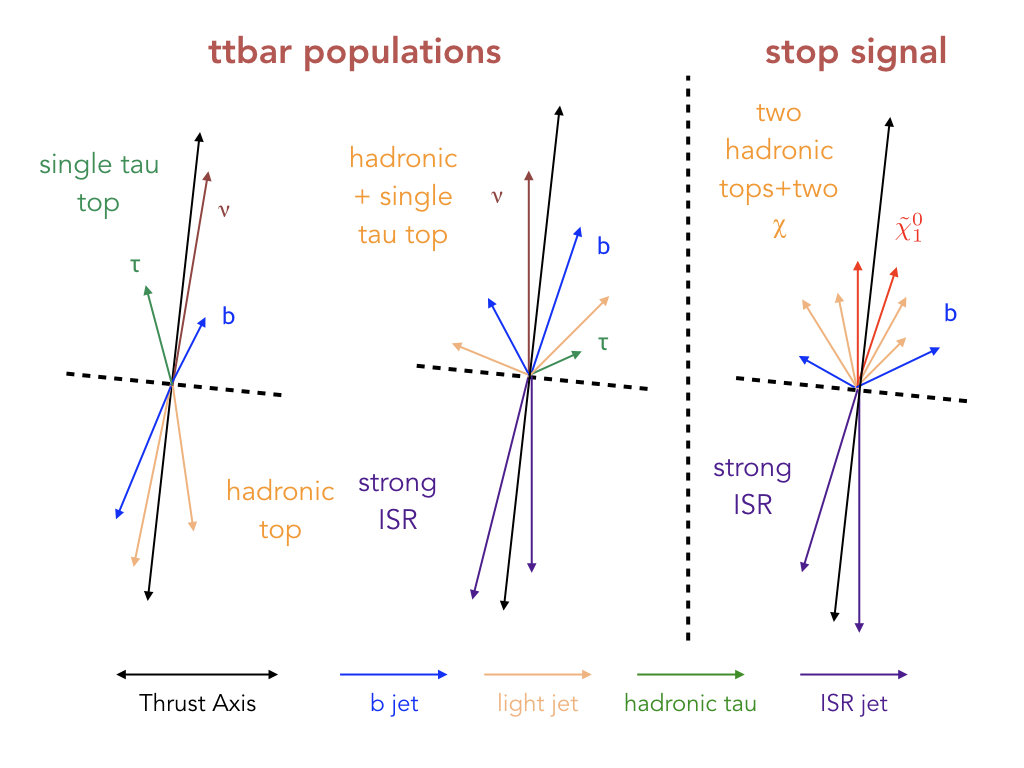
\includegraphics[width=0.65\textwidth]{./figures/strategy/ttbar_vs_signal.png}
\caption{\label{fig:ttbar:3pop}{Basic depiction of the kinematics of the two ttbar populations and stop plus strong ISR events after 0 lepton pre-selection }}
\end{figure}

\indent We can immediately see that the signal has a  significantly higher jet multiplicity and total energy in the hemisphere with the $\MET$ than the top/anti-top back-to-back population in ttbar.  Indeed, the signal has 6 jets originating from the two hadronic tops in the hemisphere with $\MET$ compared with only a single leptonic top in the top/anti-top back-to-back ttbar population.   The ttbar plus strong ISR population looks more signal like as it has higher jet multiplicity and energy in the \MET hemisphere. However, it still has less total energy then that of the signal.  \\

\indent By placing requirements on the jet multiplicity and total energy in the hemisphere with $\MET$ we are able to reject over 99 percent of ttbar events with less than 400 GeV of true ISR $\pt$.  Acceptance of ttbar events increase with true ISR $\pt$ but only asymptotically.  Even at 1200 GeV of true ISR $\pt$, a ttbar event which already passed zero lepton preselection only has a 35 percent chance of passing the additional SR selection.  \\

\indent  After pre-selection, 90 percent of all ttbar events belong to the top/anti-top back-to-back population.  Boosting one top against the other top simply requires less center-of-mass energy than boosting both tops with additional strong ISR. \\

\indent After SR selection, only approximately 10 percent of all ttbar events have true ISR $\pt$ less than 400 $\gev$.  A back-of-the-envelope calculation shows that ttbar events need around 600 $\gev$ of ISR $\pt$ in order to boost the neutrino past the 250 $\gev$ $\met$ selection if both tops started at rest.  Such high ISR $\pt$ is required because the neutrino must share the ISR $\pt$ with the 5 other particles in the ttbar decay.  This completely agrees with the true ISR $\pt$ distribution in SR which peaks around 550-600 $\gev$ for ttbar background in SR.  The ttbar true ISR $\pt$ distribution in SR can be seen in figure \ref{fig:ttbar:SR:trueISRpt}.  \\

\begin{figure}[h!]
  \centering
	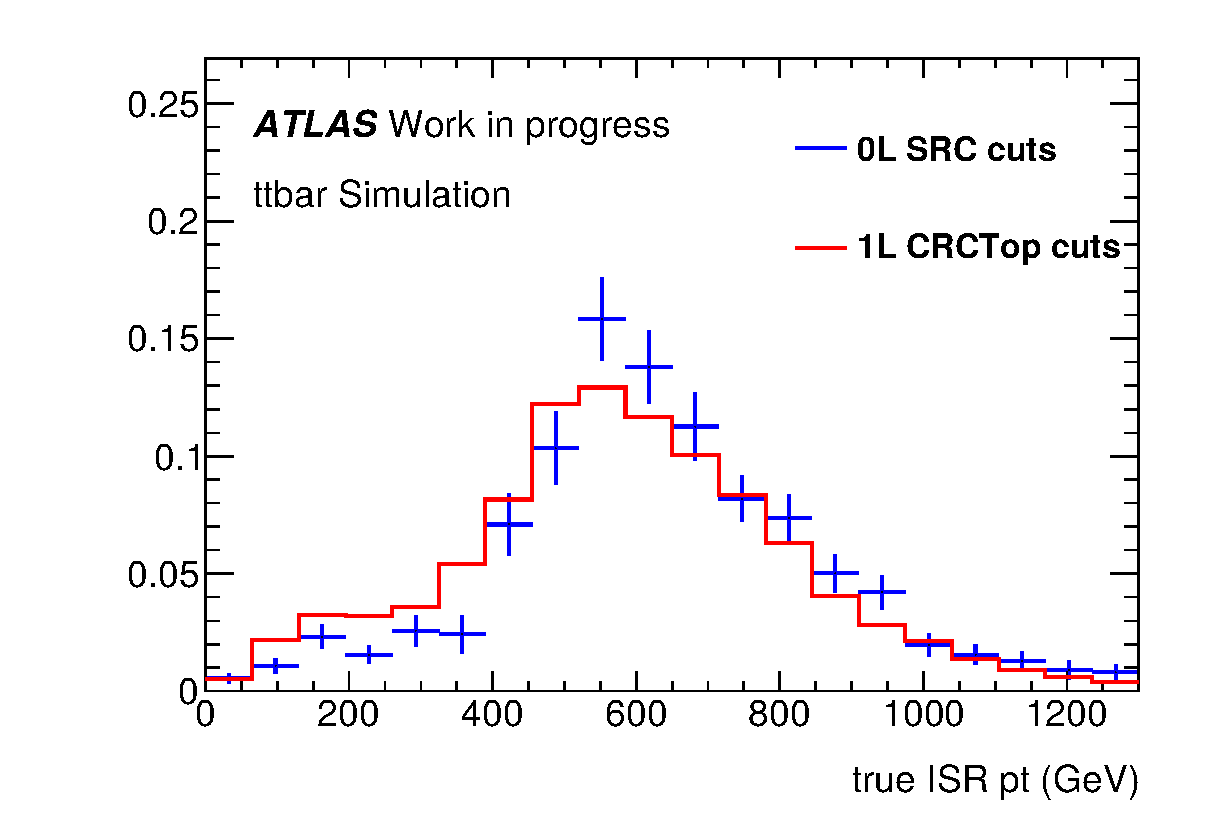
\includegraphics[width=0.65\textwidth]{./figures/ttbar/truePtISR_SRC_CRC_compare.eps}
\caption{\label{fig:ttbar:SR:trueISRpt}{Distribution of true ISR $\pt$ for ttbar that survive the signal selections}}
\end{figure}

\indent The analysis works by isolating ttbar with at least 550 $\gev$ of ISR $\pt$.  In comparison, a 400 $\gev$ stop requires only 440 $\gev$ of ISR $\pt$ to pass the 250 $\gev$ $\met$ requirement.  We effectively gain an order of magnitude in signal to background ratio (S/B) due to the lower required ISR $\pt$ in signal.  \\

\indent At the same time, we gain another factor of 5 improvement in S/B simply by working in the zero lepton channel.  In SR, the stops decay mainly via the all-hadronic decay channel with a 44 percent branching fraction.  In comparison, 80 percent of ttbar background in SR decay via the hadronic tau channel with a branching fraction of approximately 10 percent.  \\

\indent The $\met$ and ISR correlations in both direction and magnitude further improve the S/B ratio by another factor of 5 to 10 depending on the stop mass.  When combined, we are able to overcome the original 300 times difference in product cross section between the 400 $\gev$ stop and SM ttbar.  \\

\indent As the stop mass increases, the required ISR $\pt$ in signal decreases according to $m_{\stop}/m_{\ninoone}$, further increasing the accepted signal differential cross section, even if the signal production cross section is dropping.  At the same time, the signal will peak at higher $\RISR$ ratios where background contributions are lower.  In this way, the analysis is able to maintain sensitivity across a wide range of stop masses despite rapidly dropping signal production cross section at high stop masses.  \\

\indent After zero lepton preselection, the S/B ratio is $1\:40$ for a stop mass of 400 GeV.  After signal region selection, the S/B ratio improves to approximately $2\:1$ for the same mass point.  A quantitative breakdown of SR selection and yields is given in section \ref{sec:SR:Selections} and \ref{sec:SR:Yields}.  \\

\indent At the same time, the same kinematic selections on jet multiplicity and total energy are also difficult for sub-dominant backgrounds such as $W$+jets, $Z$+jets, single top and QCD multijet to satisfy.  It is in general difficult for these other processes to produce such high jet multiplicity and total energy in the same half of the event as the $\MET$.   Processes such as $W$+jets and $Z$+jets normally have the $\MET$ recoiling against other energetic jets.  Therefore, energetic jets in these processes tend to lie in the hemisphere opposite the $\MET$.  Total sub-dominant background contributions to SR is around 10 to 30 percent depending on $\RISR$ region.  \\

%\section{Kinematic Variables Definitions}
%\label{sec:SR:Definitions}



%\indent We construct variables that measure kinematic properties of both the ISR and sparticle hemispheres.  The variables used in SR definition are listed below: \\

%\begin{description}
%\item [\boldmath \nBJetS:] number of b-tagged jets associated with the sparticle hemisphere.
%\item [\boldmath \nJetS:] number of jets associated with the sparticle hemisphere.
%\item [\boldmath \pTSBZero:] $\pt$ of the leading b-jet in the sparticle hemisphere.
%\item [\boldmath \pTSFour:] $pt$ of the fourth jet ordered in $\pt$ in the sparticle hemisphere.
%\item [\boldmath \dPhiISRMET:] angular separation in $\phi$ of the ISR and the $\met$ in the CM frame.
%\item [\boldmath \pTISR:] \pt\ of the ISR system, evaluated in the CM frame.
%\item [\boldmath \mS:] transverse mass between the whole sparticle system and $\met$.
%\item [\boldmath \mV/\mS:] ratio of the transverse mass of the only the visible part of the sparticle system without $\met$ and the whole sparticle system including $\met$.
%\item [\boldmath \rISR:] Ratio between invisible system ($\met$ in CM frame) and $\pTISR$
%\end{description}



\section{Signal Region Kinematic Selection}
\label{sec:SR:Selections}

\indent Kinematic Selections for Signal Region is defined in table \ref{tab:SignalRegionC}.\\

\indent The kinematic variables used are reconstructed using the recursive jigsaw method.  A detailed description of this method and variable defined can be found in section \ref{Jigsaw:ISR}.  In short, the recursive jigsaw method separates the event into two hemispheres according to the thrust axis.  The thrust axis, the axis that maximizes the amount of back-to-back $\pt$ along it, should approximate the direction of ISR and sparticle back-to-back recoil in events with strong ISR.  The hemisphere containing the $\MET$ is considered the sparticle hemisphere and the hemisphere opposite the $\MET$ is considered the ISR hemisphere.  All jets in the sparticle hemisphere are considered to have originated from one of the stop decays.  All jets in the ISR hemisphere are considered ISR jets.  The performance of this ISR identification algorithm can be found in section \ref{Jigsaw:Performance}. \\

\indent We also construct variables that measure kinematic properties of both the ISR and sparticle hemispheres.  These include $\NbV$ and $\NjV$, which describe the jet multiplicity of the sparticle system.  $\MS$, $\pTjV$, and $\pTSBZero$ are all related to the total energy in the sparticle system.  $\pTISR$ corresponds to the total $\pt$ of the ISR system.  Finally $\RISR$ and $\dphiISRI$ quantify the correlation between the ISR system and $\MET$ in both direction and magnitude. \\

\begin{table}[htpb]
  \caption{Signal region definitions, in addition to the preselection requirements presented in Table~\ref{tab:0Lcommon}. }
  \begin{center}
    \def\arraystretch{1.4}%
    \begin{tabular}{c||c|c|c|c|c} \hline\hline
      {\bf Variable} & SRC-1 & SRC-2 & SRC-3 & SRC-4 & SRC-5 \\ \hline \hline
      \nBJetS & \multicolumn{5}{c}{$\ge1$} \\
      \nJetS & \multicolumn{5}{c}{$\ge5$}  \\
      \pTISR & \multicolumn{5}{c}{$>400$ GeV}   \\ 
      \pTSBZero & \multicolumn{5}{c}{$>40\gev$}  \\ 
      \pTSFour & \multicolumn{5}{c}{$>50$ GeV}   \\ 
      \mS & \multicolumn{5}{c}{$>300\gev$}  \\ \hline
      \dPhiISRMET & \multicolumn{5}{c}{$>3.00$}  \\ \hline
      \rISR &  0.30-0.40 & 0.40-0.50 & 0.50-0.60 & 0.60-0.70 & 0.70-0.80\\  \hline \hline
    \end{tabular}
  \end{center}
  \label{tab:SignalRegionC}
\end{table}%

\indent The selections on $\nJetS$ and $\nBJetS$ ensures that the hemisphere with $\MET$ has high amounts of jet multiplicity.  These requirements are naturally satisfied in signal events because the two neutralinos go in the same direction as the six jets from the two stop decays.  However, this requirement is more difficult to satisfy for the top/anti-top back-to-back ttbar population since these events contain only a single leptonic or hadronic tau top in the same hemisphere as the $\MET$.  \\

\indent The ttbar plus strong ISR population is able to pass this selection as both the leptonic and hadronic tops are in the sparticle hemisphere.  For this reason, the main background is comprised of these events after the sparticle jet multiplicity and the $\pTISR > 400 \GeV$ requirements.  The S/B ratio is around $1\:5$ after these selections.  \\

%\indent Distribution of different kinematic variables is shown after a requirement on $\pTISR$, $\nJetS$, and $\nBJetS$ is shown in figure \ref{fig:SR:jetMultiplicity}. The ttbar MC is normalized to a 1 lepton control region with the same selections on sparticle jet multiplicity, and $\pTISR$.  All sub-dominant background are normalized to their respective CRs defined in section \ref{sec:Bkg:sub}.\\

%\begin{figure}[htbp]
%  \begin{center}
%    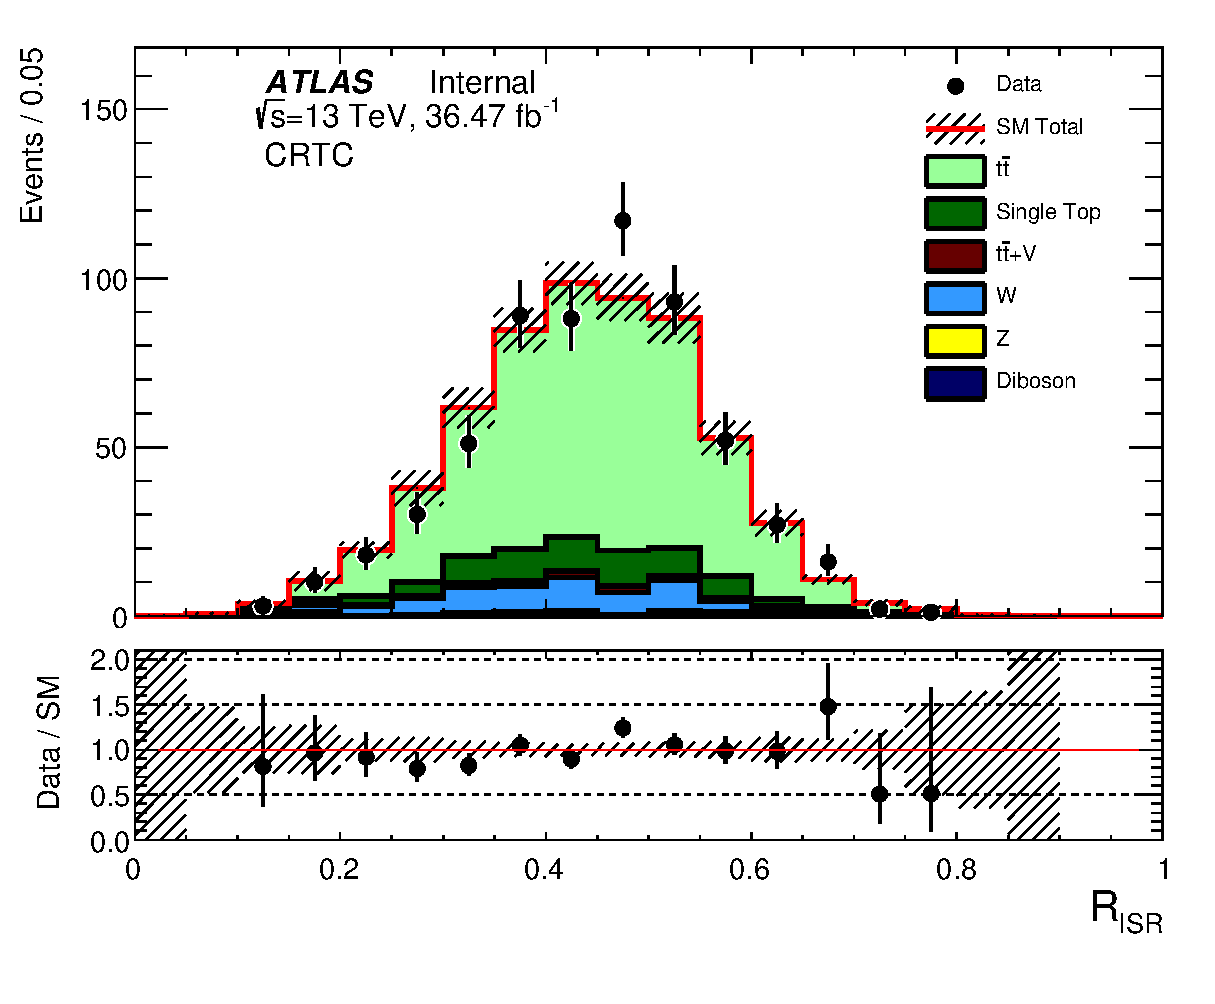
\includegraphics[width=0.45\textwidth]{figures/ttbar/postfit/CA_RISR_CRTopC}
%    \includegraphics[width=0.45\textwidth]{figures/ttbar/postfit/CA_pTISR_CRTopC}
%    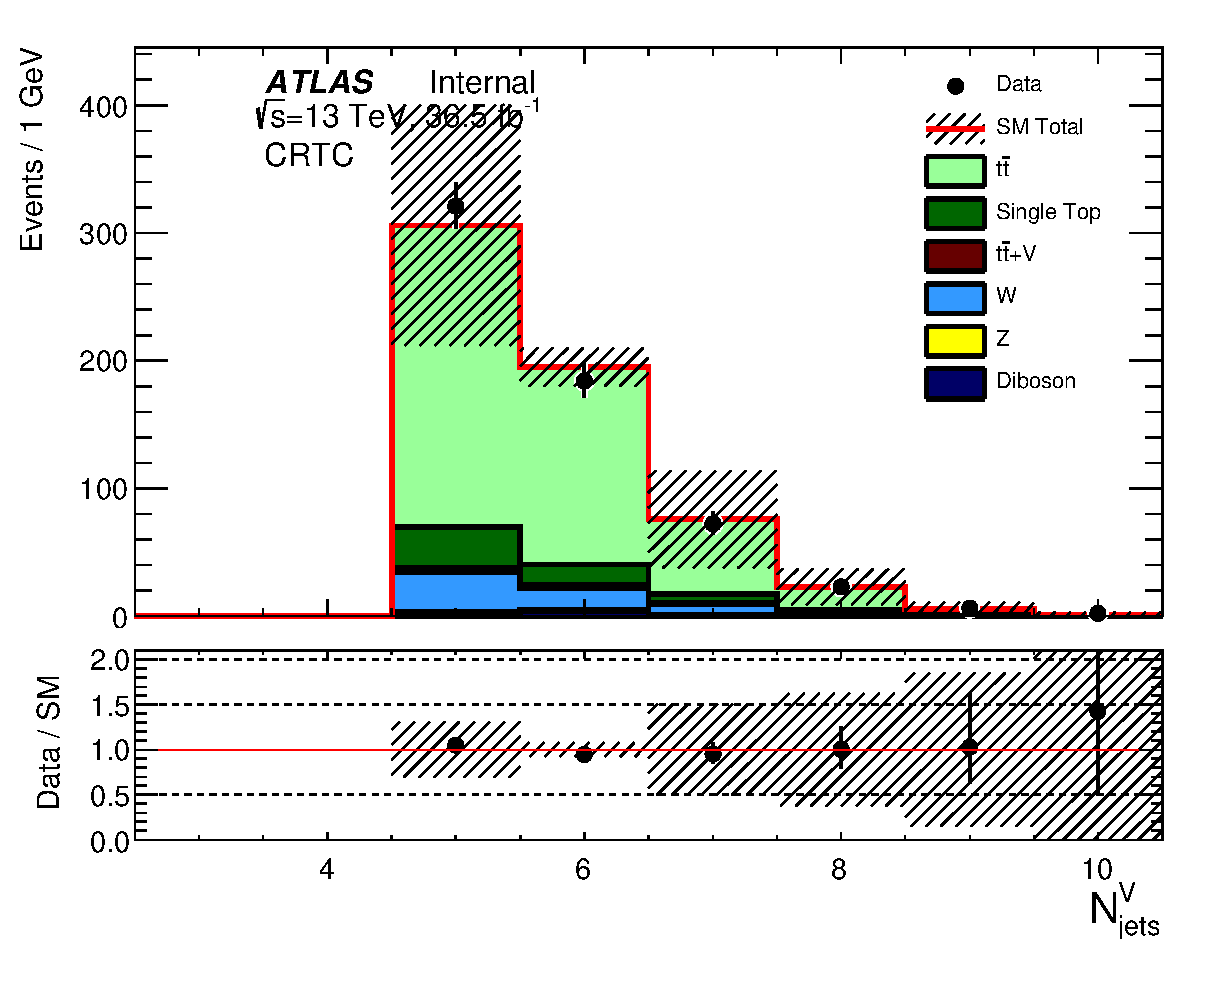
\includegraphics[width=0.45\textwidth]{figures/ttbar/postfit/CA_NjV_CRTopC}
%    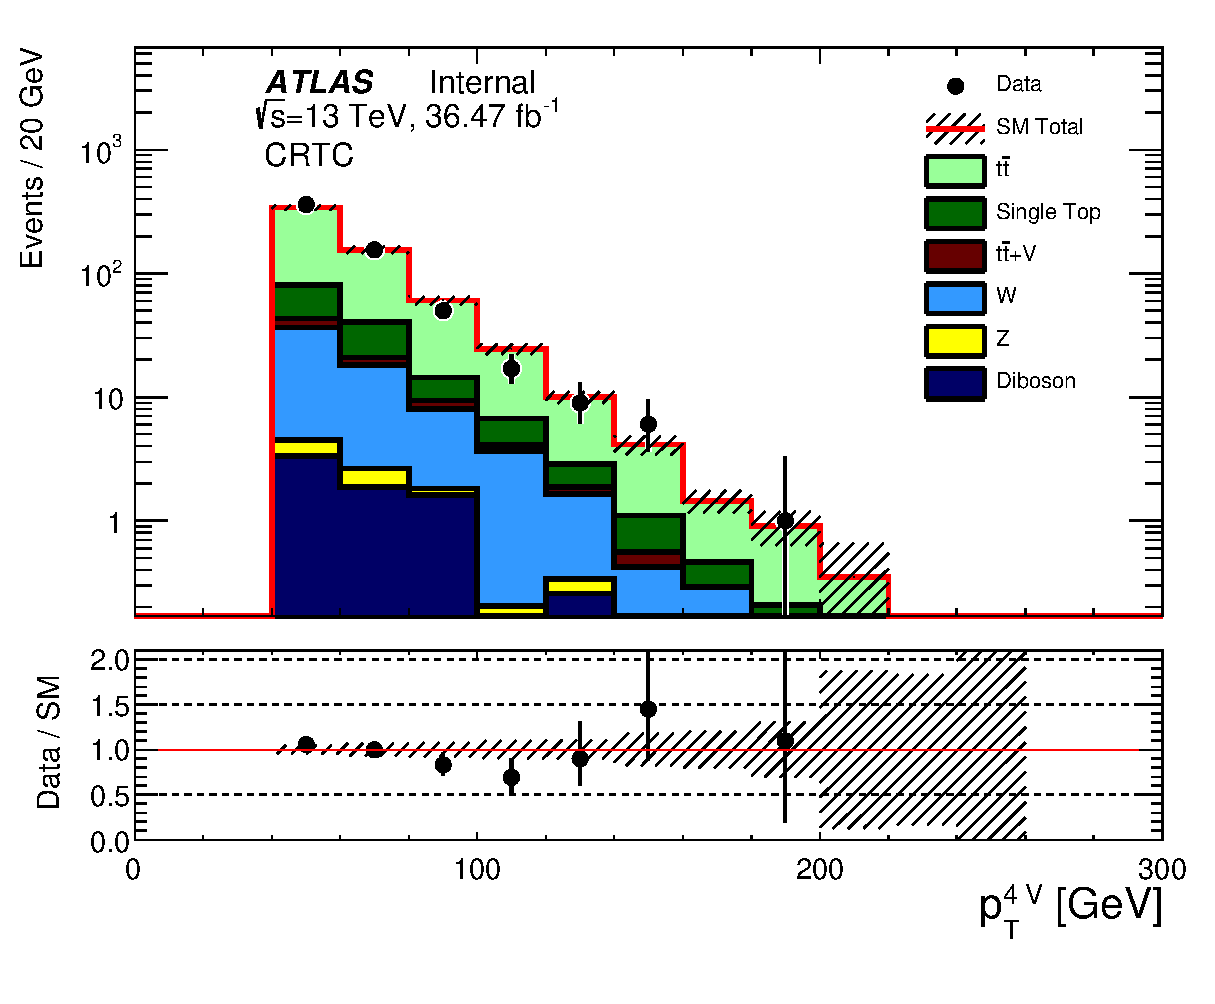
\includegraphics[width=0.45\textwidth]{figures/ttbar/postfit/CA_pTjV4_CRTopC_log}
%    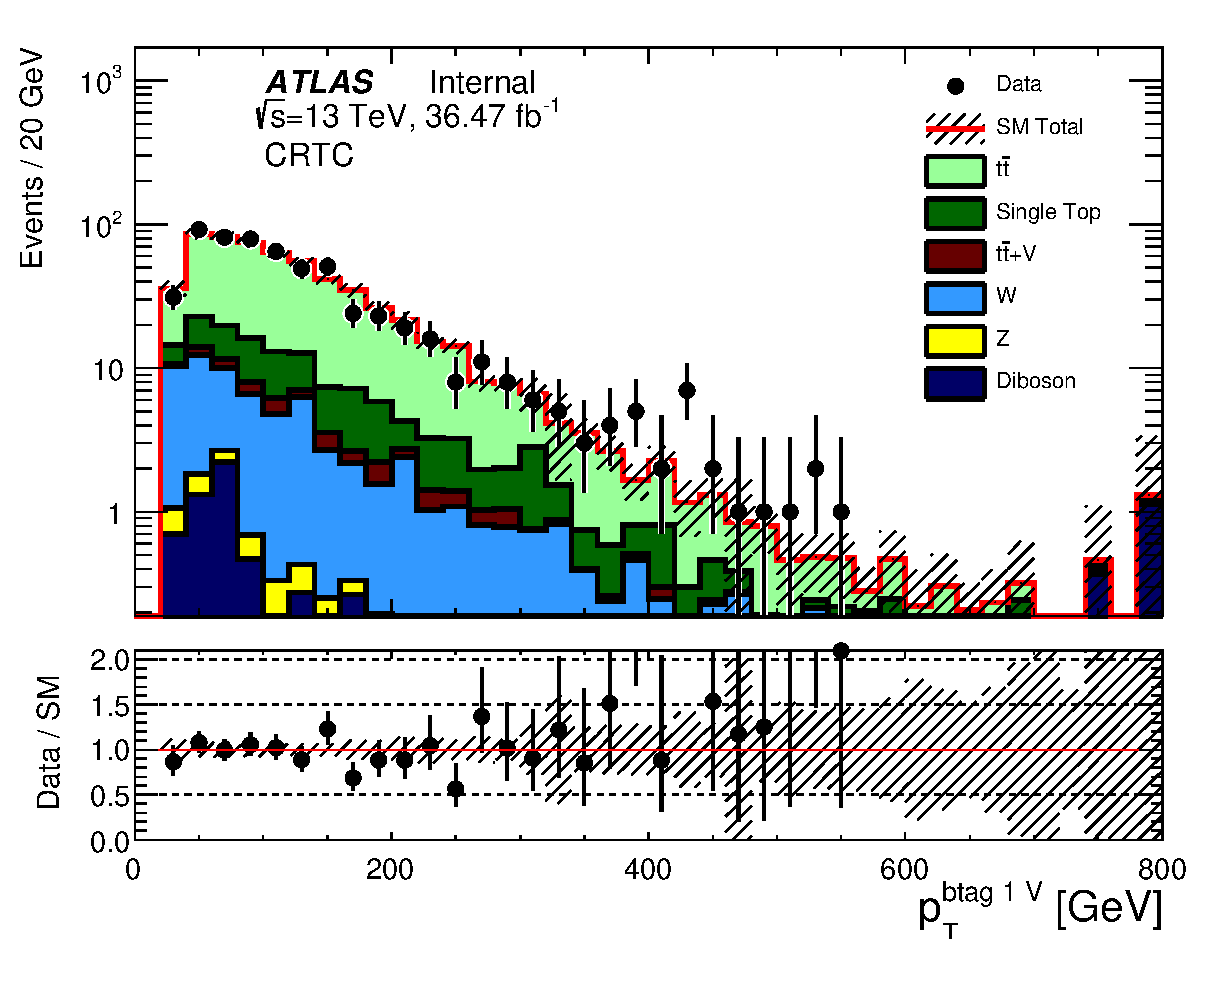
\includegraphics[width=0.45\textwidth]{figures/ttbar/postfit/CA_pTbV1_CRTopC_log}
%        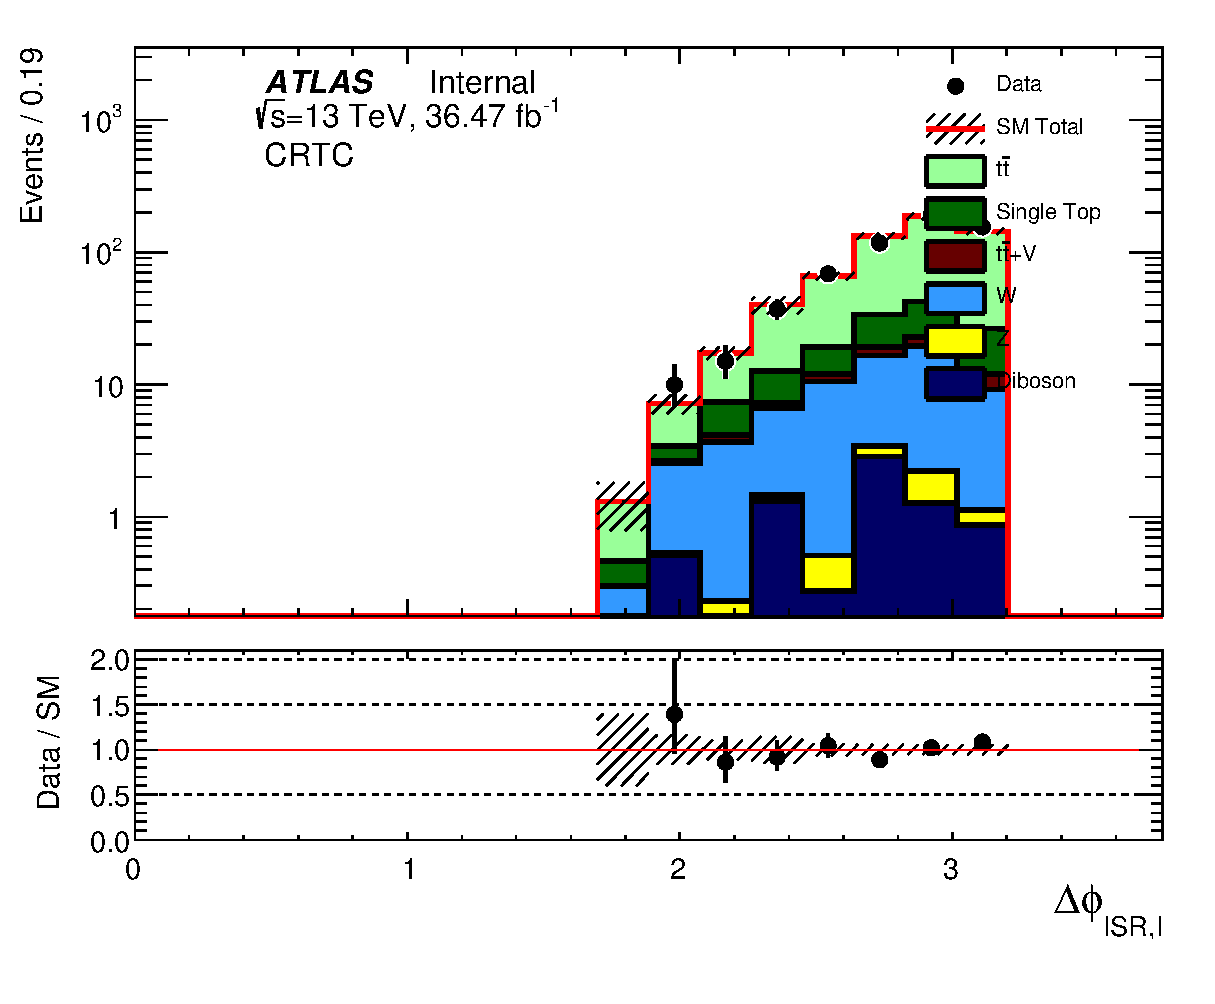
\includegraphics[width=0.45\textwidth]{figures/ttbar/postfit/CA_dphiISRI_CRTopC_log}
%  \end{center}
%  \caption{{\bf NEEDS PLOTS} Distributions for 0 lepton preselection plus $\pTISR > 400 \gev$, $\nBJetS\ge1$  and $\nJetS\ge5$ with \intlumi\ \ifb\ of data. The ratio between data and MC is shown in the bottom panel. The hashed area in both the top and lower panel represent the uncertainty due to MC statistics and detector plus theoretical systematic uncertainties}
%  \label{fig:SR:jetMultiplicity}
%\end{figure}

\indent Next, we make a requirement on the total energy of the sparticle system.  The total transverse mass of the sparticle system, $\mS$, must be greater then $300 \gev$ and $\pTSFour$, $\pt$ of the 4th highest $\pt$ jet in the sparticle system, must be greater then $50 \gev$.  $\pTSBZero$, the highest $\pt$ b-jet in the sparticle system, must also be greater then $40 \gev$.   \\

\indent In general, the signal with two fully hadronic tops has more energy in the sparticle hemisphere then ttbar.  The top/anti-top back-to-back recoil population is nearly eliminated by these selections.  Of the ttbar events that passed zero lepton preselection, less then 2 percent of ttbar events with true ISR $\pt$ less then $400 \gev$ pass these additional requirements.   Even for ttbar events with greater then $600 \gev$ of true ISR $\pt$, the selection efficiency remain at approximately 35 percent.  S/B ratio improves to around $1\:2$ after these selections. \\

%\indent Distribution of various kinematic variables after sparticle jet multiplicity, $\pTISR$, and sparticle energy requirement is shown in figure \ref{fig:SR:sparticleEnergy}.  The ttbar MC is normalized to a 1 lepton control region with the same selections on sparticle jet multiplicity, $\pTISR$, and sparticle energy requirement.  All sub-dominant background are normalized to their respective CRs defined in section \ref{sec:Bkg:sub}.\\
%\begin{figure}[htbp]
%  \begin{center}
%    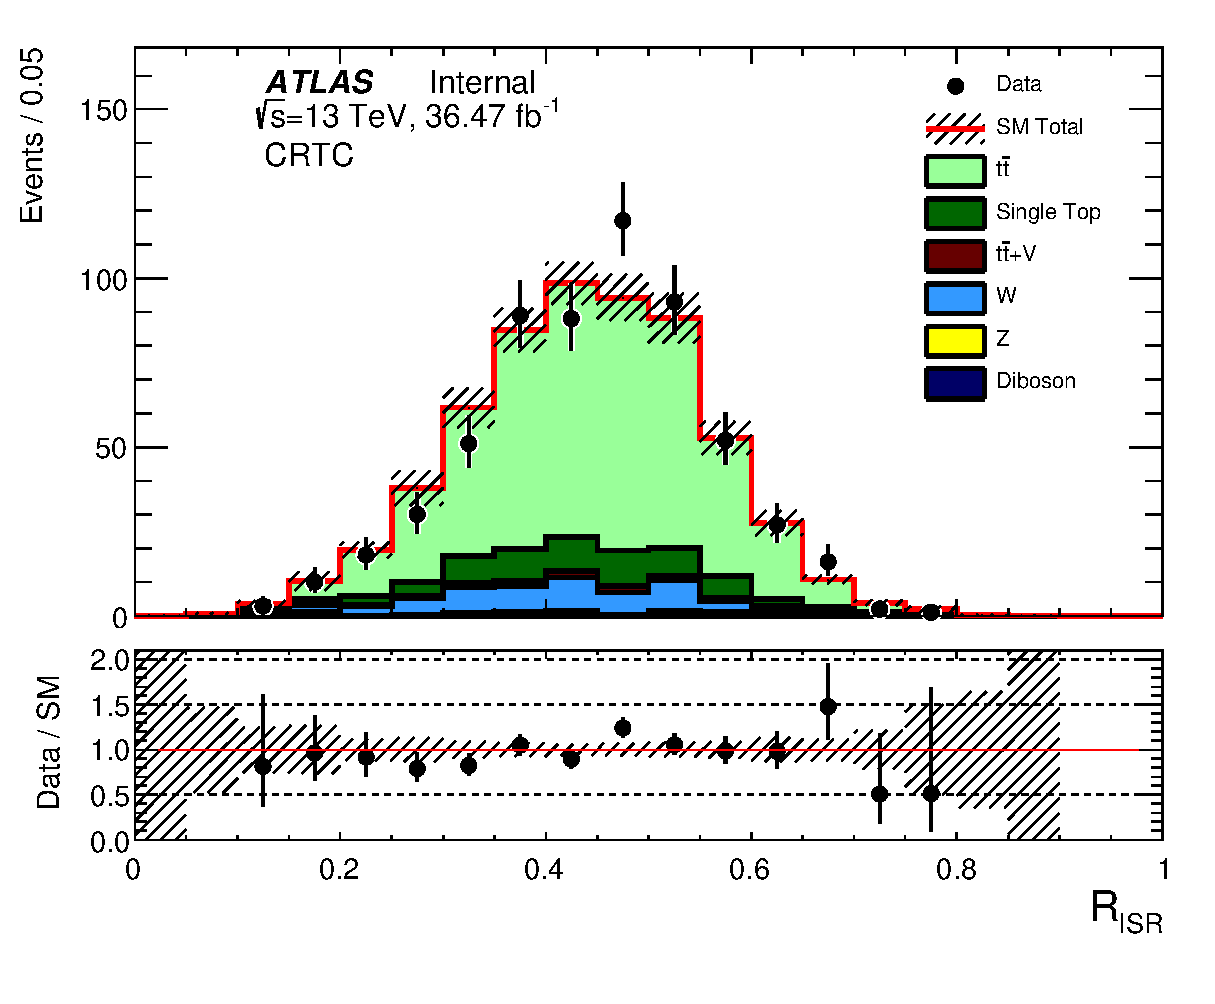
\includegraphics[width=0.45\textwidth]{figures/ttbar/postfit/CA_RISR_CRTopC}
%    \includegraphics[width=0.45\textwidth]{figures/ttbar/postfit/CA_pTISR_CRTopC}
 %   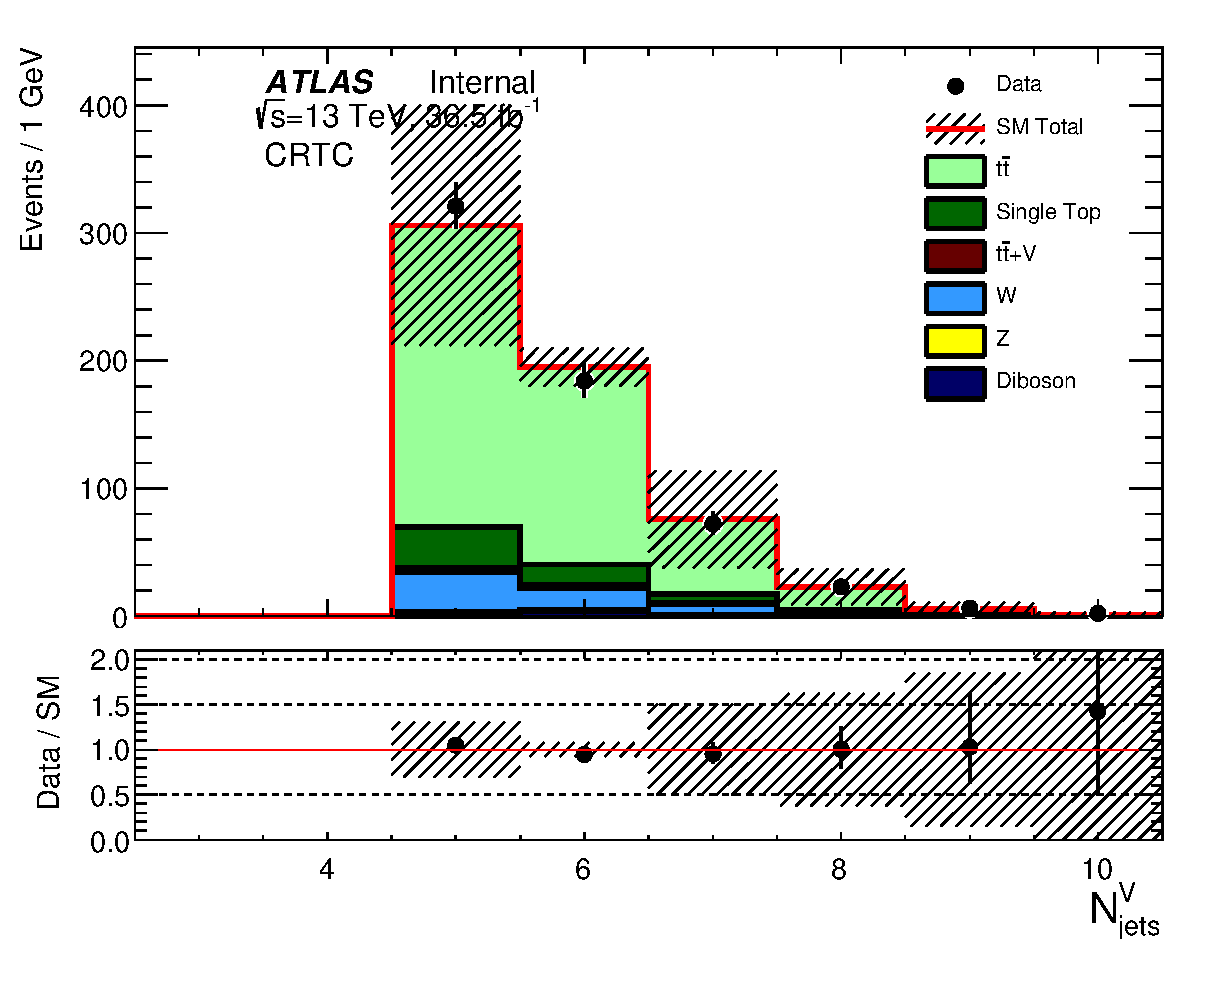
\includegraphics[width=0.45\textwidth]{figures/ttbar/postfit/CA_NjV_CRTopC}
 %   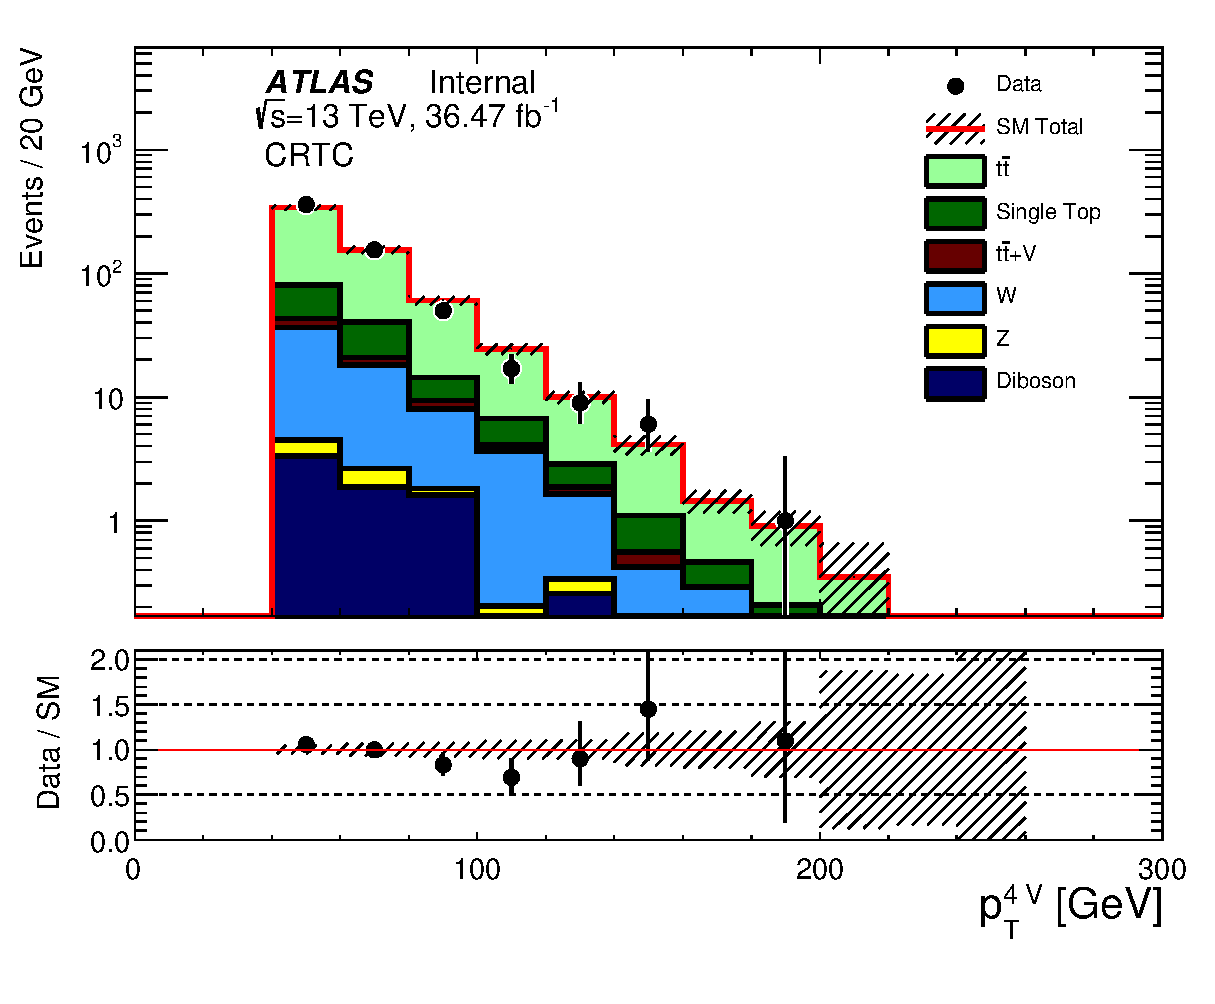
\includegraphics[width=0.45\textwidth]{figures/ttbar/postfit/CA_pTjV4_CRTopC_log}
 %   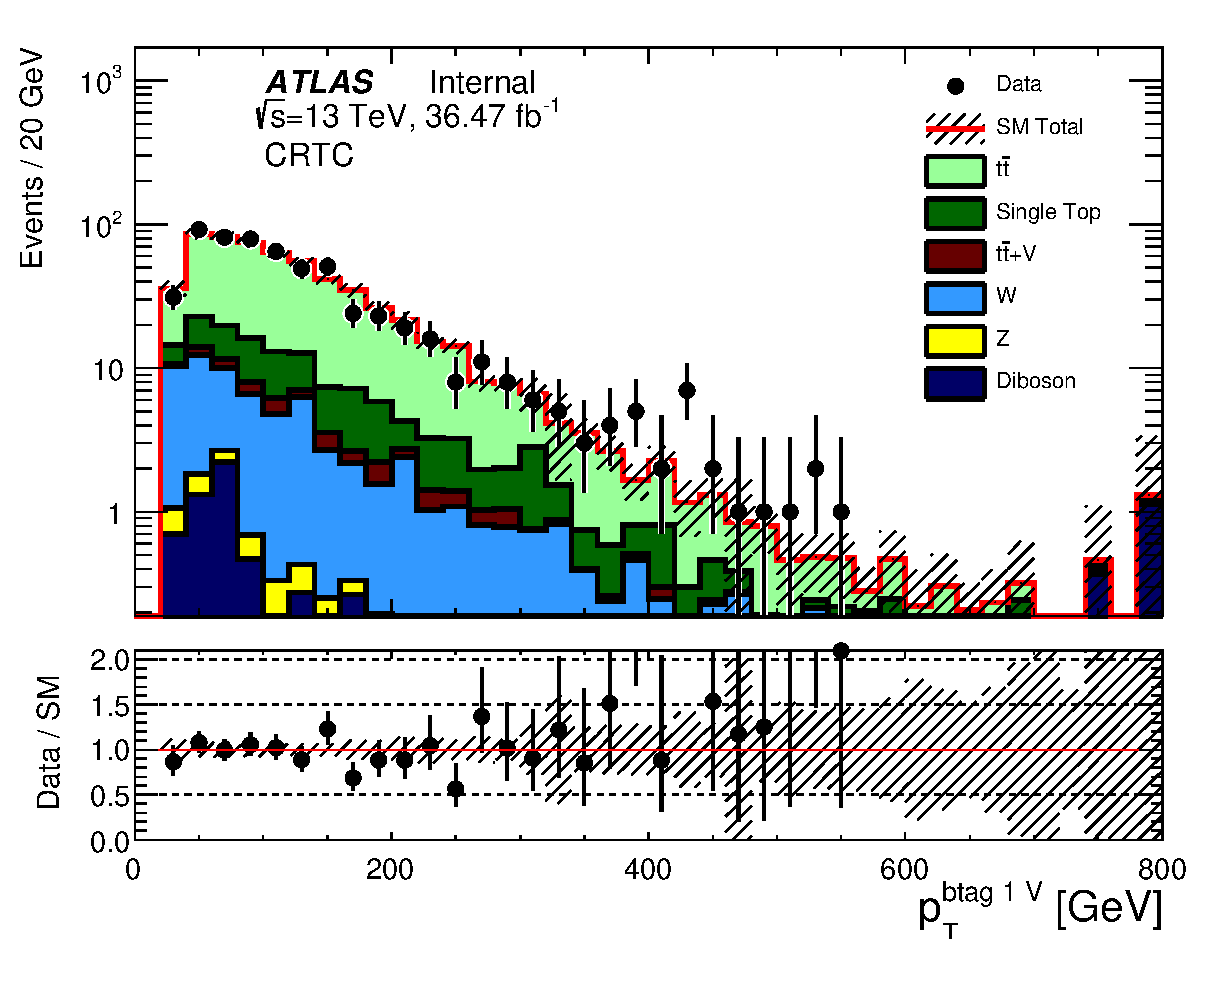
\includegraphics[width=0.45\textwidth]{figures/ttbar/postfit/CA_pTbV1_CRTopC_log}
%  \end{center}
%  \caption{{\bf NEEDS PLOTS} Distributions for 0 lepton preselection plus sparticle jet multiplicity, $\pTISR$, and sparticle total energy requirement with \intlumi\ \ifb\ of data. The ratio between data and MC is shown in the bottom panel. The hashed area in both the top and lower panel represent the uncertainty due to MC statistics and detector plus theoretical systematic uncertainties}
%  \label{fig:SR:sparticleEnergy}
%\end{figure}

\indent Lastly we make selections based on the correlations between the $\MET$ and ISR systems.  $\dPhiISRMET > 3.0$ ensures the $\MET$ and ISR systems are back-to-back.  The ISR system and $\MET$ must be nearly back-to-back in signal because the neutralino gains momenta mainly from ISR.  On the other hand, the neutrino in SM ttbar gains significant momentum from the top decay and its correlation with ISR is not as strong. The is also true for sub-dominant backgrounds including $W$+jet and single top. \\

\indent The distribution of $\dPhiISRMET$ with all previous selections on sparticle jet multiplicity and sparticle system energy applied is shown in figure \ref{fig:SR:dphiISRMET}.   %The ttbar MC is normalized to a 1 lepton control region with the same selections on sparticle jet multiplicity, $\pTISR$, and sparticle energy requirement.  All sub-dominant background are normalized to their respective CRs defined in section \ref{sec:Bkg:sub}. \\

\begin{figure}[htbp]
  \begin{center}
     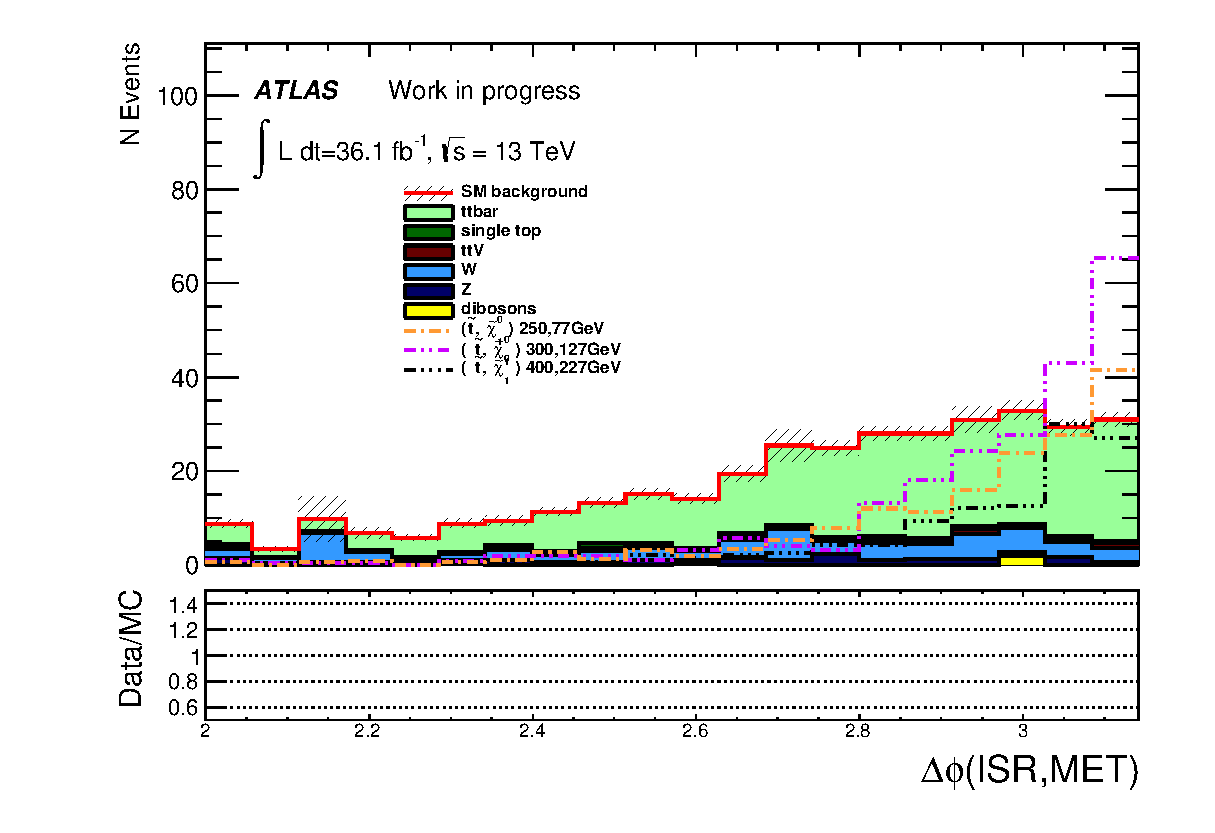
\includegraphics[width=0.80\textwidth]{figures/plotSR/SR_ND1_dphiISRI_6SR.eps}
  \end{center}
  \caption{$\dPhiISRMET$ distributions for the zero lepton preselection plus sparticle jet multiplicity, $\pTISR$, and sparticle total energy requirement with \intlumi\ \ifb\ of data. The ratio between data and MC is shown in the bottom panel. The hashed area in both the top and lower panel represent the uncertainty due to MC statistics}
  \label{fig:SR:dphiISRMET}
\end{figure}

\indent The final $\RISR$ distribution after all signal selections is shown in figure \ref{fig:SR:RISR}.  This $\RISR$ distribution is then separated into $5$ bins from $0.3$ to $0.8$.  The 5 SR bins are fitted simultaneously to extract the signal strength.  We expect to receive very little signal events in $\RISR$ below 0.3 and the region is dominated by QCD background.  As such the $\RISR$ region below 0.3 is not included in the final SR fit.  \\

\begin{figure}[htbp]
  \begin{center}
     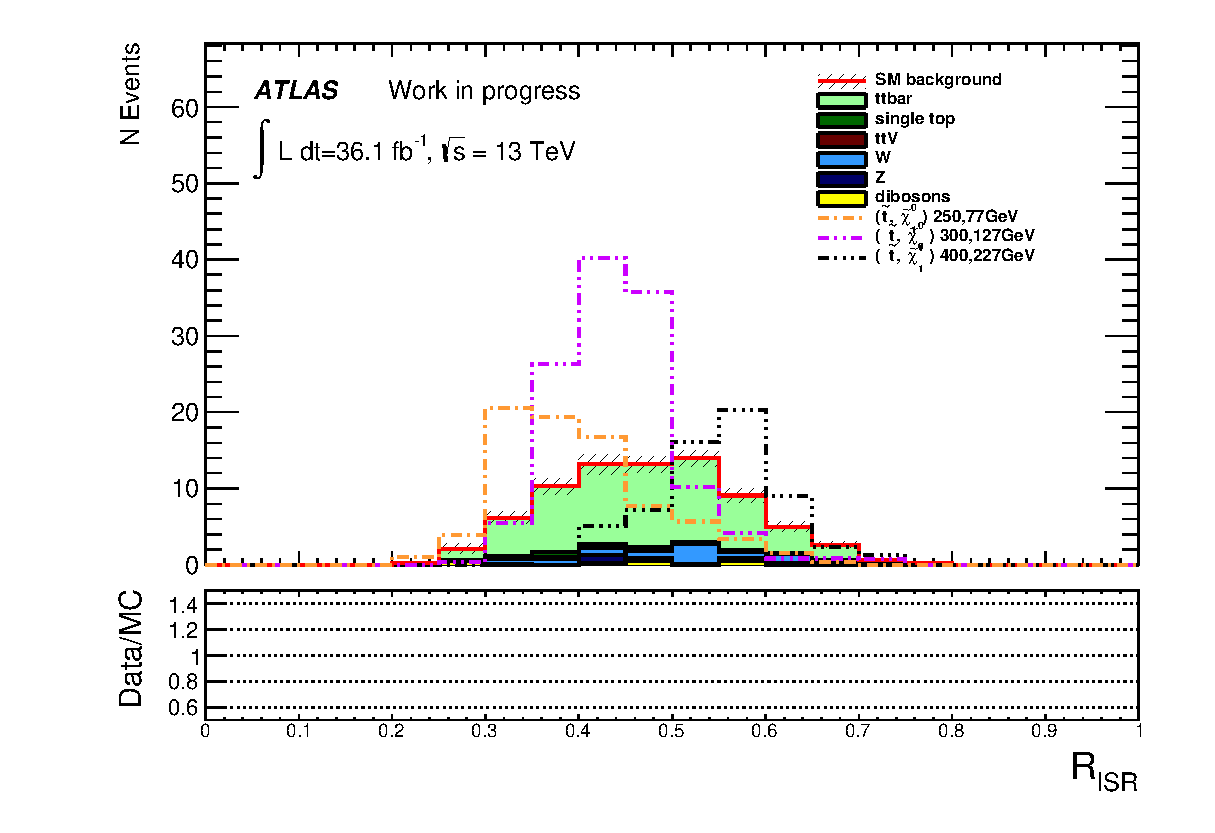
\includegraphics[width=0.80\textwidth]{figures/plotSR/SR_ND1_RISR_7SR.eps}
  \end{center}
  \caption{ $\RISR$ distribution after signal region selection with \intlumi\ \ifb\ of data. The ratio between data and MC is shown in the bottom panel. The hashed area in both the top and lower panel represent the uncertainty due to MC statistics}
  \label{fig:SR:RISR}
\end{figure}

\indent Stop samples with different stop and neutralino masses will peak in different locations in $\RISR$ with a S/B ratio of approximately $2\:1$ under the peak.  The simultaneous fit to all five bins captures this peaking feature in $\RISR$ for any stop mass.  \\

\section{Signal Region Expected Yields and Kinematic Distributions}
\label{sec:SR:Yields}

\indent The expected yields in SR are given in table \ref{tab:SRyield}.  All backgrounds have been normalized to CR defined in chapter \ref{chap:backgrounds}.  Signal yields for three example signal samples with stop, neutralino masses of $(300,127 \gev), (400,227\gev), $ and $(500,327 \gev)$ are also shown for comparison.  We achieved a $1\:1$ to $2\:1$ S/B ratio under the signal $\RISR$ peak in SR. \\

\begin{table}
  \begin{center}
    \def\arraystretch{1.4}%
    \begin{tabular}{c|c}
\hline\hline
\multicolumn{2}{c}{\bf SRC1 } \\ \hline 
Z & 0.11 $\pm$ 0.03 \\
dibosons & 0.04 $\pm$ 0.04 \\
ttbar & 1.99 $\pm$ 0.46 \\
singleTop & 0.09 $\pm$ 0.06 \\
ttV & 0.03 $\pm$ 0.04 \\
W & 0.46 $\pm$ 0.23 \\
\hline
Total MC & 2.72 $\pm$ 0.52 \\
\hline\hline
\end{tabular}

    \begin{tabular}{c|c}
\hline\hline
\multicolumn{2}{c}{\bf SRC2 } \\ \hline 
Z & 0.90 $\pm$ 0.13 \\
dibosons & 0.21 $\pm$ 0.21 \\
ttbar & 31.20 $\pm$ 1.82 \\
singleTop & 1.02 $\pm$ 0.19 \\
ttV & 0.46 $\pm$ 0.19 \\
W & 1.53 $\pm$ 0.31 \\
\hline
Total MC & 35.30 $\pm$ 1.88 \\
Data & 22.00 $\pm$ 4.69 \\
\hline
(500,327) GeV & 1.42 $\pm$ 0.26  \\
\hline
(300,127) GeV & 72.20 $\pm$ 7.29  \\
\hline
(400,227) GeV & 10.81 $\pm$ 1.00 \\
\hline\hline
\end{tabular}

    \begin{tabular}{c|c}
\hline\hline
\multicolumn{2}{c}{\bf SRC3 } \\ \hline 
Z & 0.74 $\pm$ 0.15 \\
dibosons & 0.28 $\pm$ 0.28 \\
ttbar & 20.62 $\pm$ 1.07 \\
singleTop & 1.04 $\pm$ 0.41 \\
ttV & 0.44 $\pm$ 0.11 \\
W & 1.51 $\pm$ 0.37 \\
\hline
Total MC & 24.64 $\pm$ 1.25 \\
Data & 22.00 $\pm$ 4.69 \\
\hline
 ($\mstop$, $\mLSP$) = (500,327) GeV & 6.90 $\pm$ 0.56 (1.3$\sigma$) \\
\hline
 ($\mstop$, $\mLSP$) = (300,127) GeV & 14.80 $\pm$ 2.56 (2.7$\sigma$) \\
\hline
 ($\mstop$, $\mLSP$) = (400,227) GeV & 30.01 $\pm$ 1.67 (5.2$\sigma$) \\
\hline\hline
\end{tabular}

    \begin{tabular}{c|c}
\hline\hline
\multicolumn{2}{c}{\bf SRC4 } \\ \hline 
Z & 0.45 $\pm$ 0.09 \\
dibosons & 0.00 $\pm$ 0.00 \\
ttbar & 6.95 $\pm$ 0.46 \\
singleTop & 0.62 $\pm$ 0.17 \\
ttV & 0.07 $\pm$ 0.08 \\
W & 1.53 $\pm$ 0.41 \\
\hline
Total MC & 9.61 $\pm$ 0.65 \\
Data & 1.00 $\pm$ 1.00 \\
\hline
 ($\mstop$, $\mLSP$) = (500,327) GeV & 10.53 $\pm$ 0.68 (2.9$\sigma$) \\
\hline
 ($\mstop$, $\mLSP$) = (300,127) GeV & 0.80 $\pm$ 0.57 (0.1$\sigma$) \\
\hline
 ($\mstop$, $\mLSP$) = (400,227) GeV & 8.95 $\pm$ 0.86 (2.5$\sigma$) \\
\hline\hline
\end{tabular}

    \begin{tabular}{c|c}
\hline\hline
\multicolumn{2}{c}{\bf SRC5 } \\ \hline 
Z & 0.44 $\pm$ 0.10 \\
dibosons & 0.15 $\pm$ 0.10 \\
ttbar & 6.33 $\pm$ 0.72 \\
singleTop & 0.53 $\pm$ 0.14 \\
ttV & 0.08 $\pm$ 0.08 \\
W & 1.38 $\pm$ 0.37 \\
\hline
Total MC & 8.91 $\pm$ 0.84 \\
\hline\hline
\end{tabular}

  \end{center}
  \caption{Signal Region expected discovery significance for select samples with 20\% background systematic uncertainty.}
  \label{tab:SRyield}
\end{table}

\indent Distributions of kinematic variables in SR are shown in figure \ref{fig:SR} \\

\begin{figure}[htbp]
  \begin{center}
    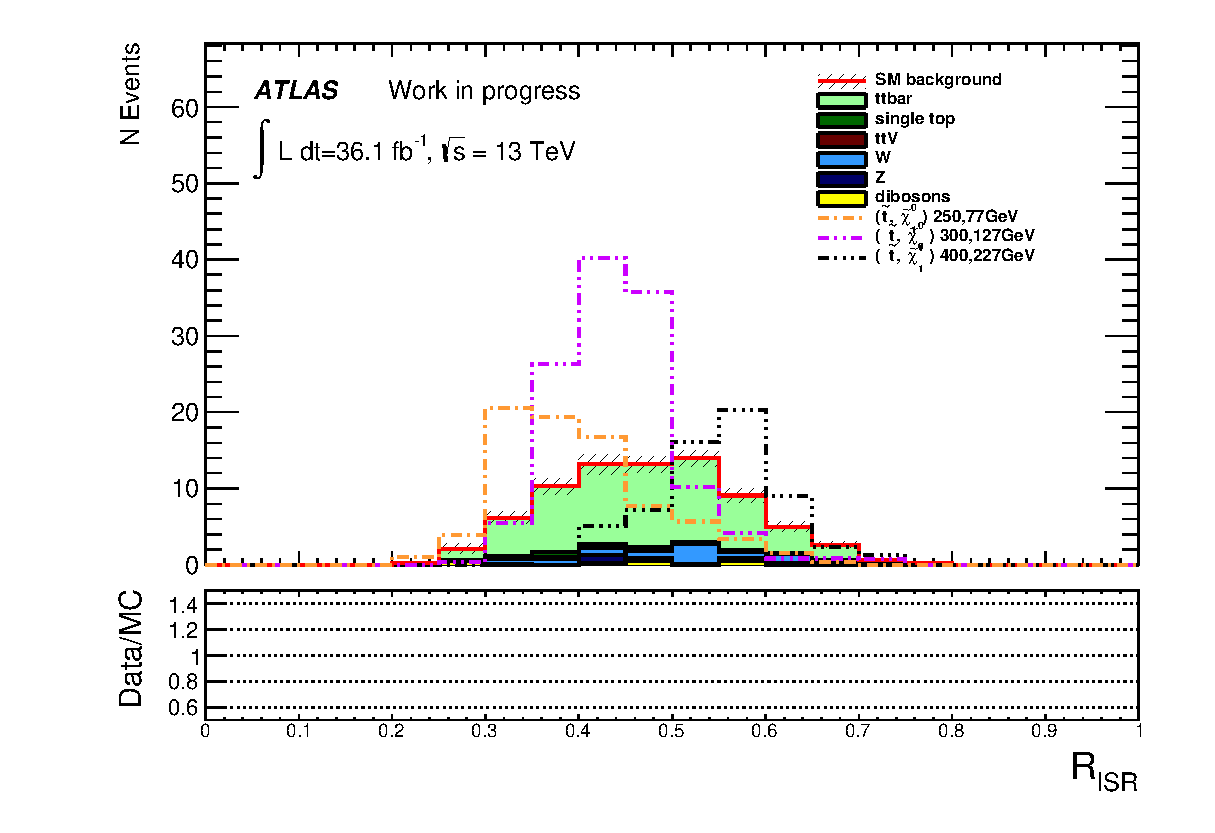
\includegraphics[width=0.45\textwidth]{figures/plotSR/SR_ND1_RISR_7SR.eps}
    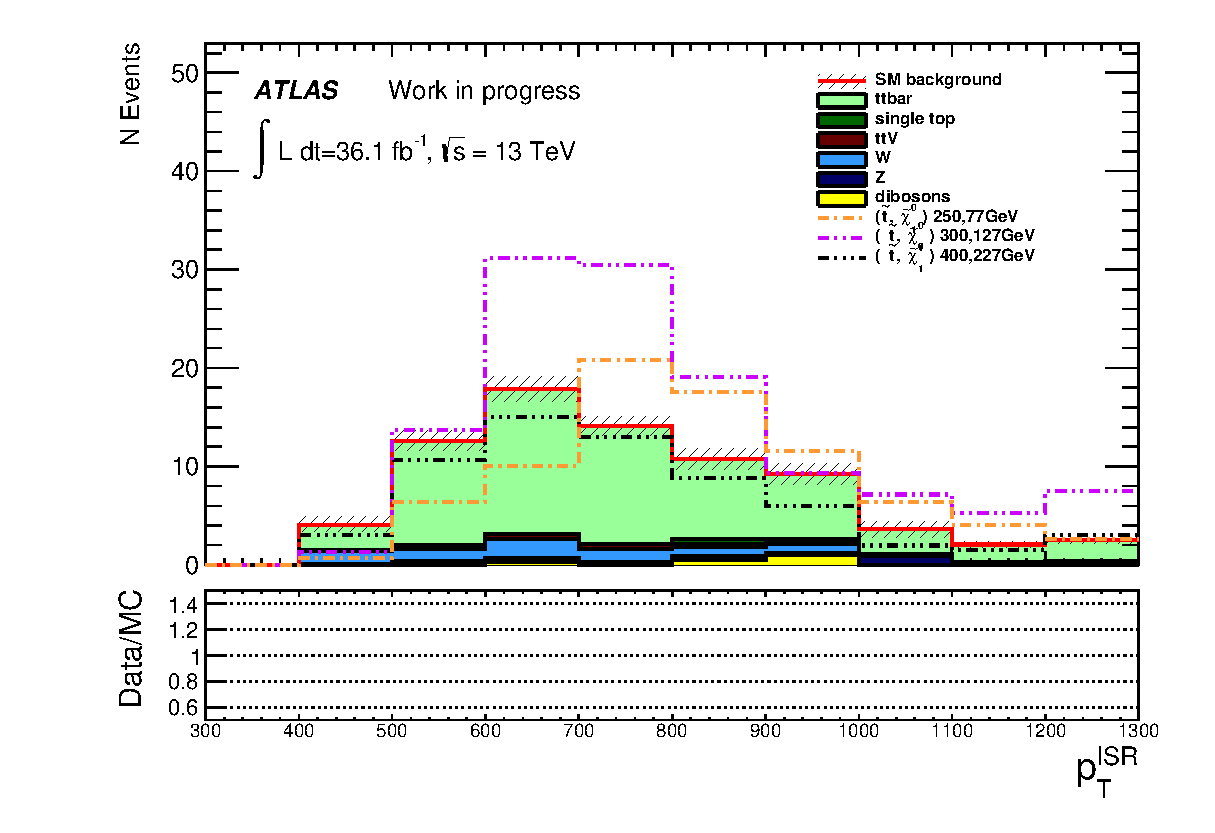
\includegraphics[width=0.45\textwidth]{figures/plotSR/SR_ND1_PTISR_7SR.eps}
    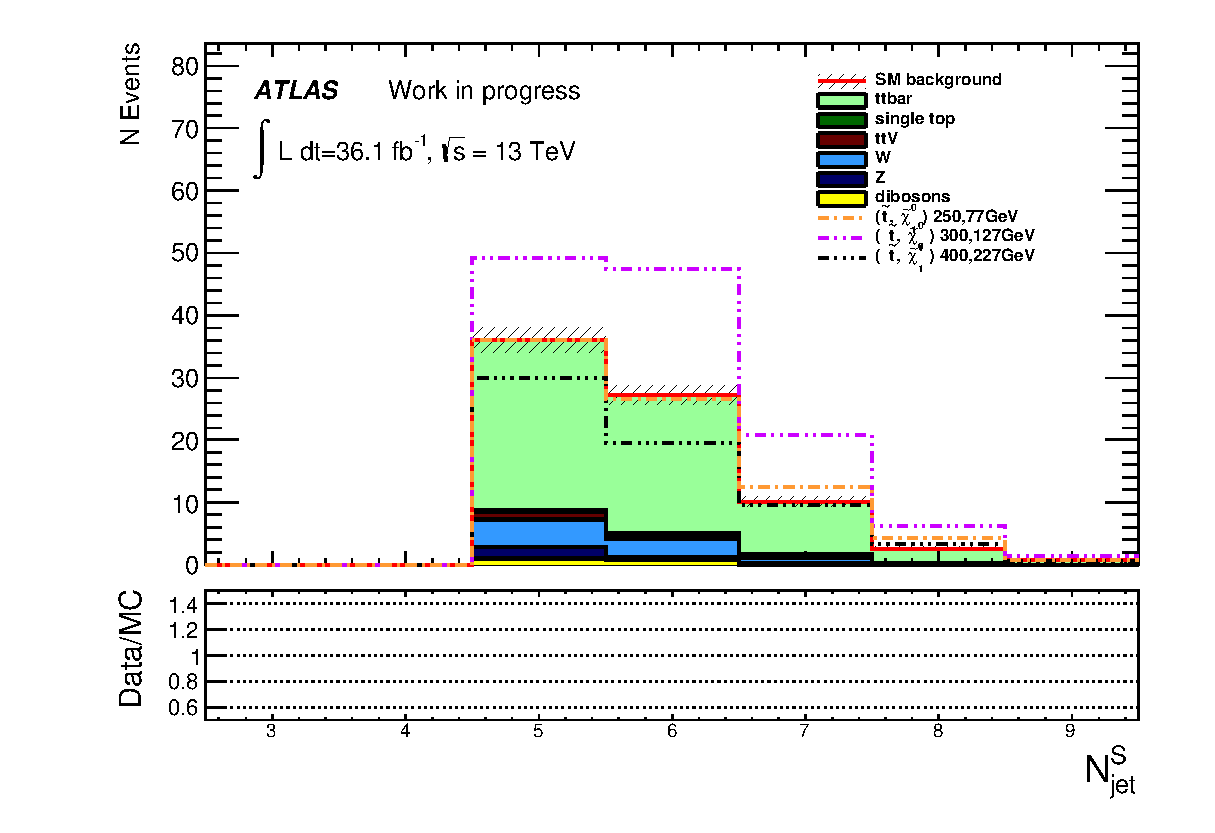
\includegraphics[width=0.45\textwidth]{figures/plotSR/SR_ND1_NjV_7SR.eps}
    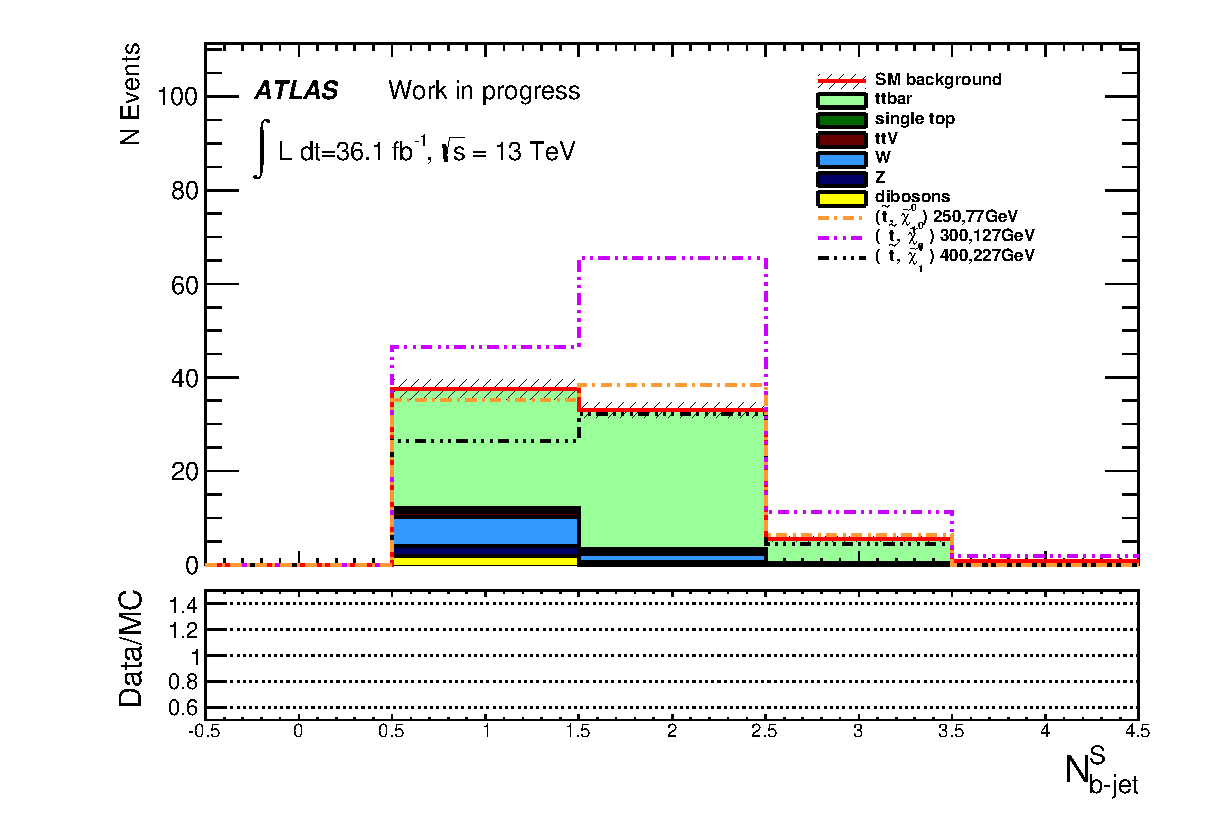
\includegraphics[width=0.45\textwidth]{figures/plotSR/SR_NbV_7SR.eps}
    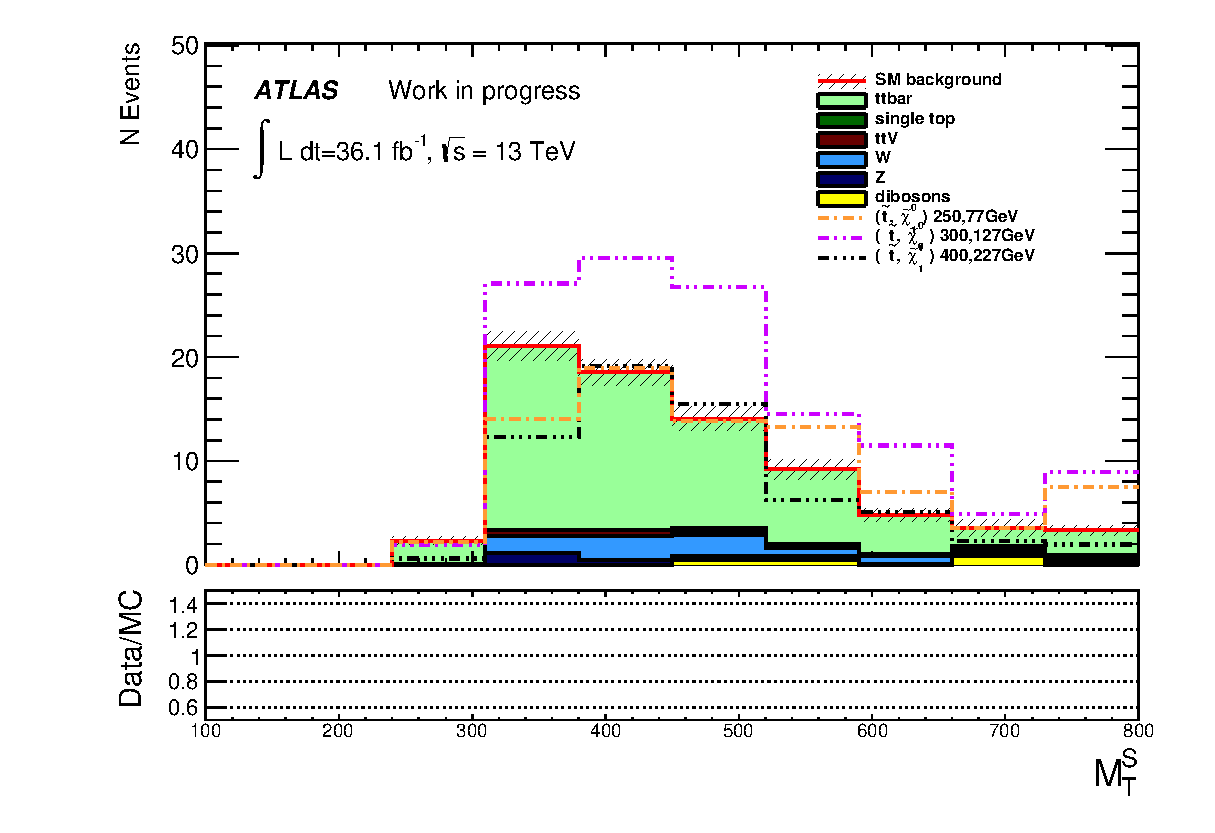
\includegraphics[width=0.45\textwidth]{figures/plotSR/SR_ND1_MS_7SR.eps}
    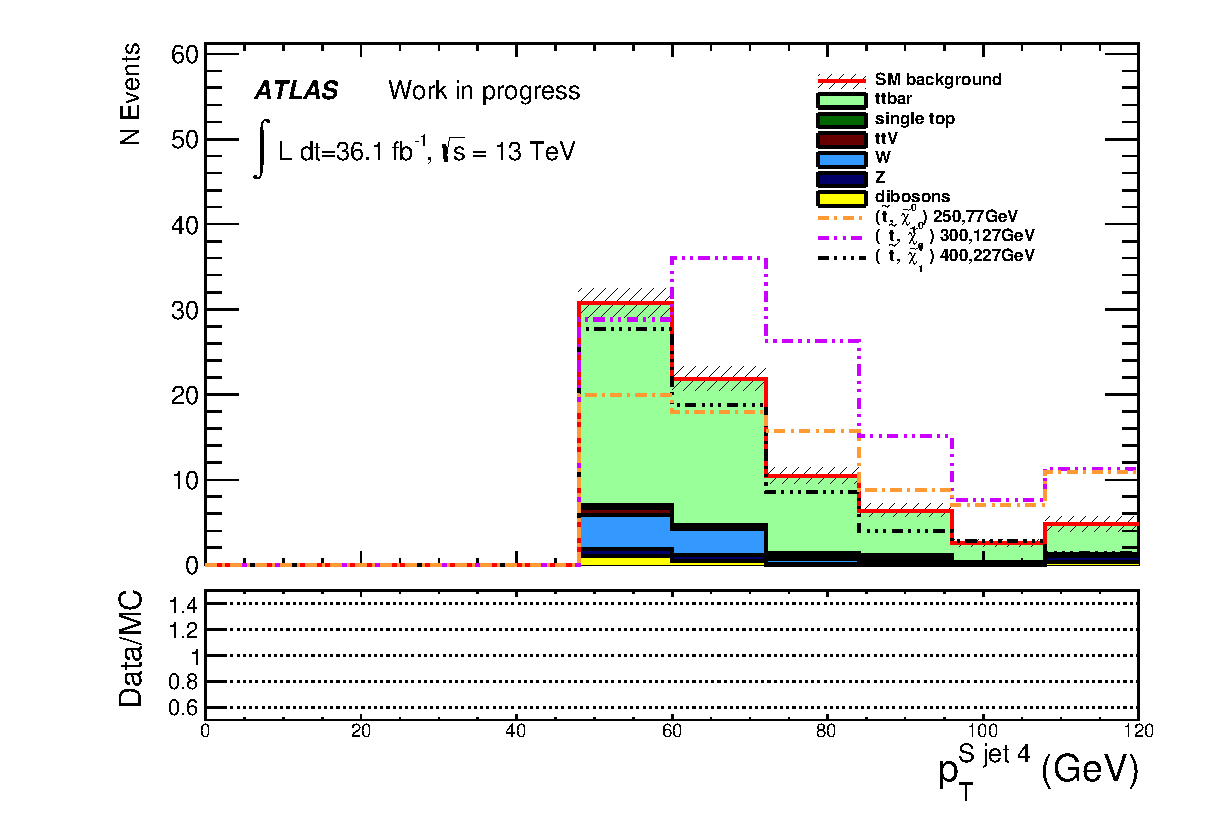
\includegraphics[width=0.45\textwidth]{figures/plotSR/SR_ND1_pTjV4_7SR.eps}
    \caption{ Distributions for signal region selection. The ratio between data and MC is shown in the bottom panel. The hashed area in both the top and lower panel represent the uncertainty due to MC statistics.  QCD background estimation is not included.  }
    \end{center}
  \label{fig:SR}
\end{figure}

\section{Signal Region Background Composition}
\label{sec:Bkg:Compositiion}

The dominant background in all signal region bins is SM ttbar.  ttbar accounts for $85$ percent of all backgrounds in the signal region.  The next most prevalent background is W+jets which can reach up to 15 percent in high $\RISR$ bins. The breakdown of background composition is given in table \ref{tab:SRBkg} \\

\begin{table}[htpb]
  \begin{center}
    \def\arraystretch{1.4}%
    \begin{tabular}{c||c|c|c|c|c|c|} \hline\hline
      \RISR Range & 0.2-0.3 & 0.3-0.4 & 0.4-0.5 & 0.5-0.6 & 0.6-0.7 & 0.7-0.8 \\  \hline
      t\tbar  &  & & & & & \\  \hline
      $W$+jets &  & & & & & \\  \hline 
      $Z$+jets  &  & & & & & \\  \hline 
      Single top & & & & & & \\ \hline
      QCD & & & & & & \\ \hline
      dibosons  & & & & & & \\ \hline \hline
    \end{tabular}
  \caption{Standard Model Background Composition in the Signal Region ~\ref{tab:SRBkg}.   }
  \end{center}
  \label{tab:SignalRegion}
\end{table}%


